\documentclass[12pt]{article}
\usepackage[utf8]{inputenc}
\usepackage[T1]{fontenc}
\usepackage[polish]{babel}
\usepackage{geometry}
\usepackage{tabularx}
\usepackage[table,xcdraw,dvipsnames]{xcolor}
\usepackage{tabularx}
\usepackage{color}
\usepackage{subfig}
\usepackage{sidecap}
\usepackage{wrapfig}
\usepackage{float}
\usepackage{enumerate}
\usepackage{graphicx}
\usepackage{multirow}
\usepackage{hyperref}
\usepackage{titlesec}
\usepackage{amsmath}
\usepackage{anyfontsize}
\usepackage{indentfirst}
\usepackage{listings}
\usepackage{multicol}
\usepackage{pgfplots}
\usepackage{fancyhdr}

\newgeometry{tmargin=1.8cm,bmargin=1.8cm,lmargin =1.8cm,rmargin=1.8cm}
\begin{document}


\begin{table}[H]
    \centering
    \renewcommand{\arraystretch}{1.5}
    \begin{tabularx}{\textwidth}{|X|X|}
    \hline
    \multicolumn{2}{|c|}{\large\textbf{Notatka służbowa nr 1}} \\ \hline
    Temat:          & Sterownik Siemens S7-1200    \\ \hline
    Wykonanie:      & Zuzanna Mejer, 259382   \\ \hline
    Termin zajęć:   & poniedziałek TP, 10:55  \\ \hline  
    Data:           & 14.11.2022    \\ \hline
    \end{tabularx}
    \end{table}

\section{Cel ćwiczenia}
Celem ćwiczenia było zaznajomienie się z obsługą sterownika PLC Siemens Simatic S7-1200. Podczas ćwiczenia korzystano z programu TIA Portal 11, w którym należało skonfigurować sterownik oraz napisać program w języku drabinkowym. Program miał składać się z dwóch podprogramów - mnożenia dwóch liczb oraz licznika. 

\section{Uruchomienie oprogramowania i konfiguracja sterownika}
Przed rozpoczęciem pracy ze sterownikiem, należało uruchomić i skonfigurować oprogramowanie i sterownik. W tym celu wykonano poniższe czynności.
\begin{enumerate}
    \item Uruchomiono program TIA Portal 11. Po ukazaniu się strony startowej, stworzono nowy projekt i wybrano opcję ,,skonfiguruj urządzenie'' (\textit{,,Configure a device''}). Na poniższym rysunku przedstawiono stronę startową programu.
    \begin{figure}[H]
        \centering
        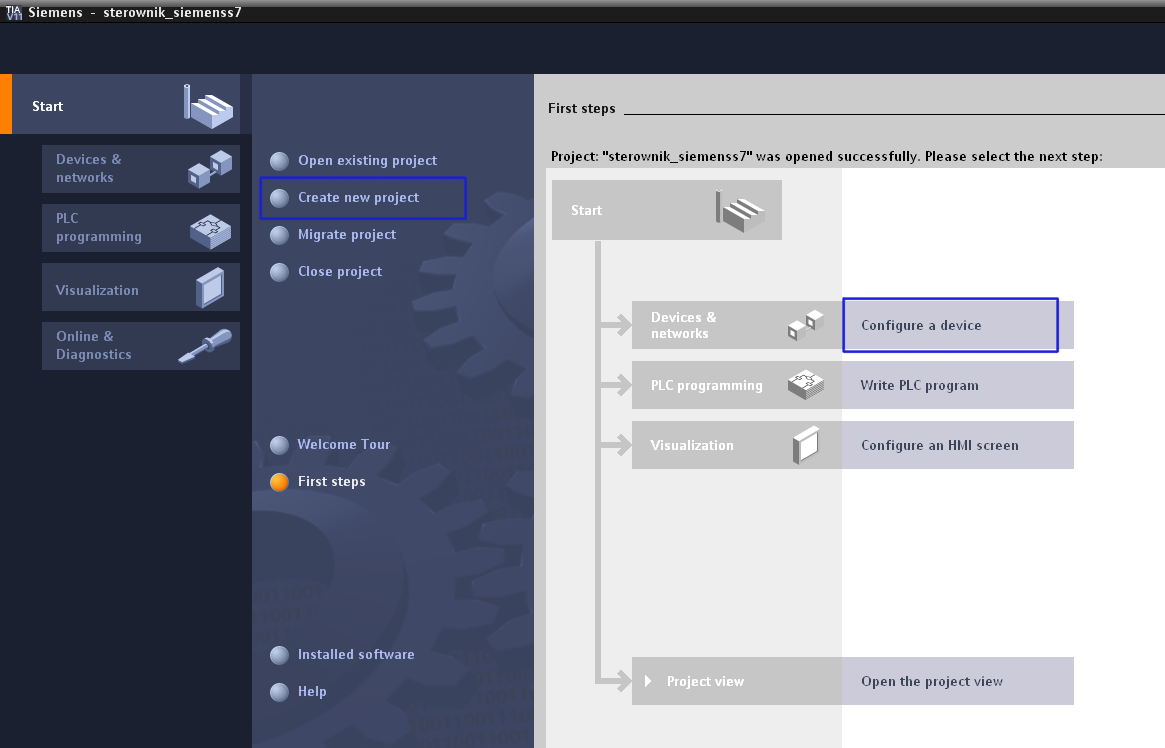
\includegraphics[scale=0.3]{./zdj/strona_startowa.png}
        \caption{Strona startowa programu TIA Portal 11}
    \end{figure}

    \item Następnie w ramach konfiguracji sprzętowej sterownika wybrano opcję ,,Dodaj nowe urządzenie'' (\textit{,,Add new device''}) w zakładce \textit{,,Devices and networks''} (rys. \ref{cpu}). Wybrano opcję \textit{PLC}, następnie z opcji dostępnych rodzajów jednostek centralnych CPU wybrano odpowiedni - CPU 1214 AC/DC/Rly z indeksem: 6ES7 214-1BE30-0XB0. 
    \begin{figure}[H]
        \centering
        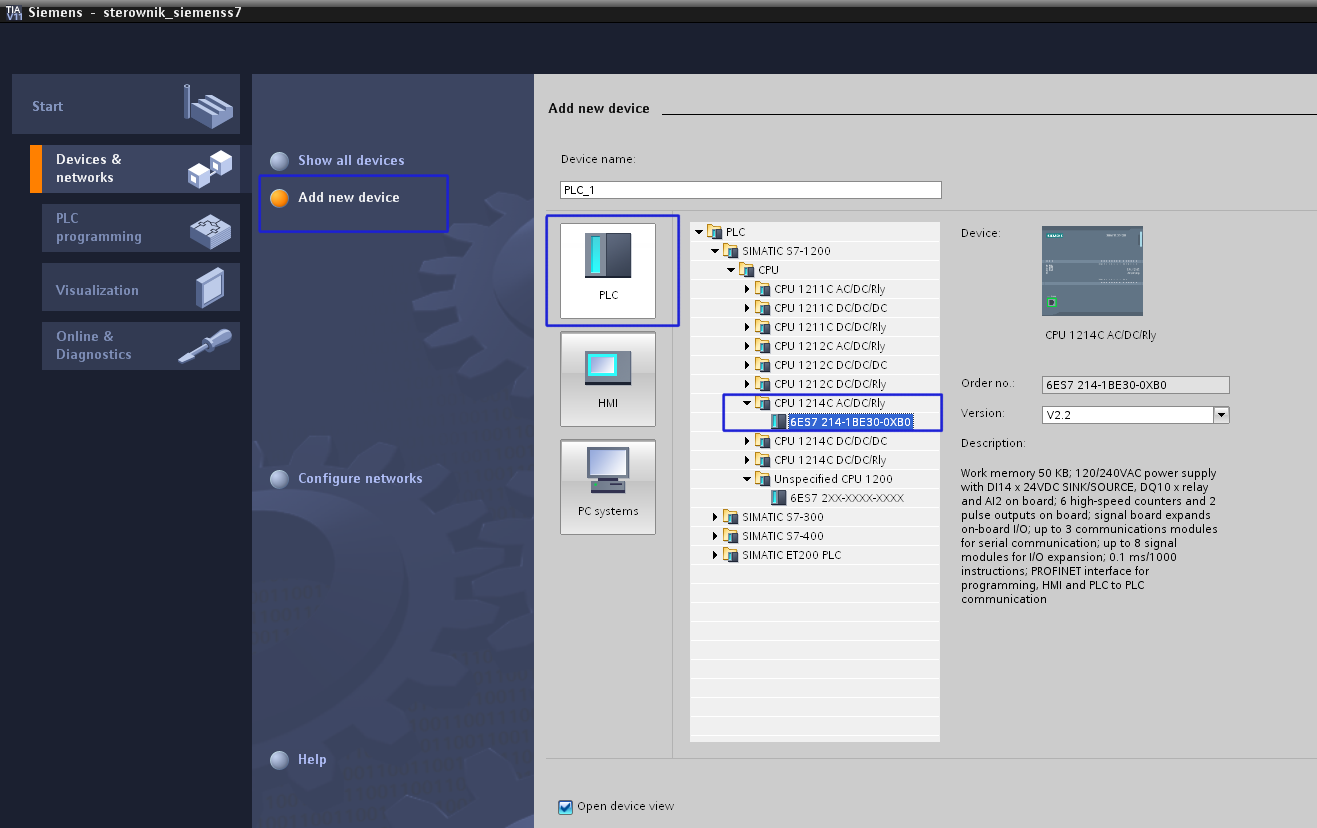
\includegraphics[scale=0.3]{./zdj/add_device.png}
        \caption{Dodawanie nowego urządzenia - zdefiniowanie CPU i indeksu}
        \label{cpu}
    \end{figure}

    \item Po dodaniu nowego urządzenia do projektu w automatycznie otwartym oknie \textit{,,Device view''} (w zakładce \textit{,,Device configuration''} okna \textit{,,Project tree''}) (rys. \ref{device view}), należało uzupełnić konfigurację sterownika o kartę sygnałową AQ1x12 bits (rys. \ref{aq1}). W tym celu należało odpowiednio wybraną z katalogu opcję przeciągnąć i upuścić w wyznaczone miejsce na modelu sterownika w programie.
    \begin{figure}[H]
        \centering
        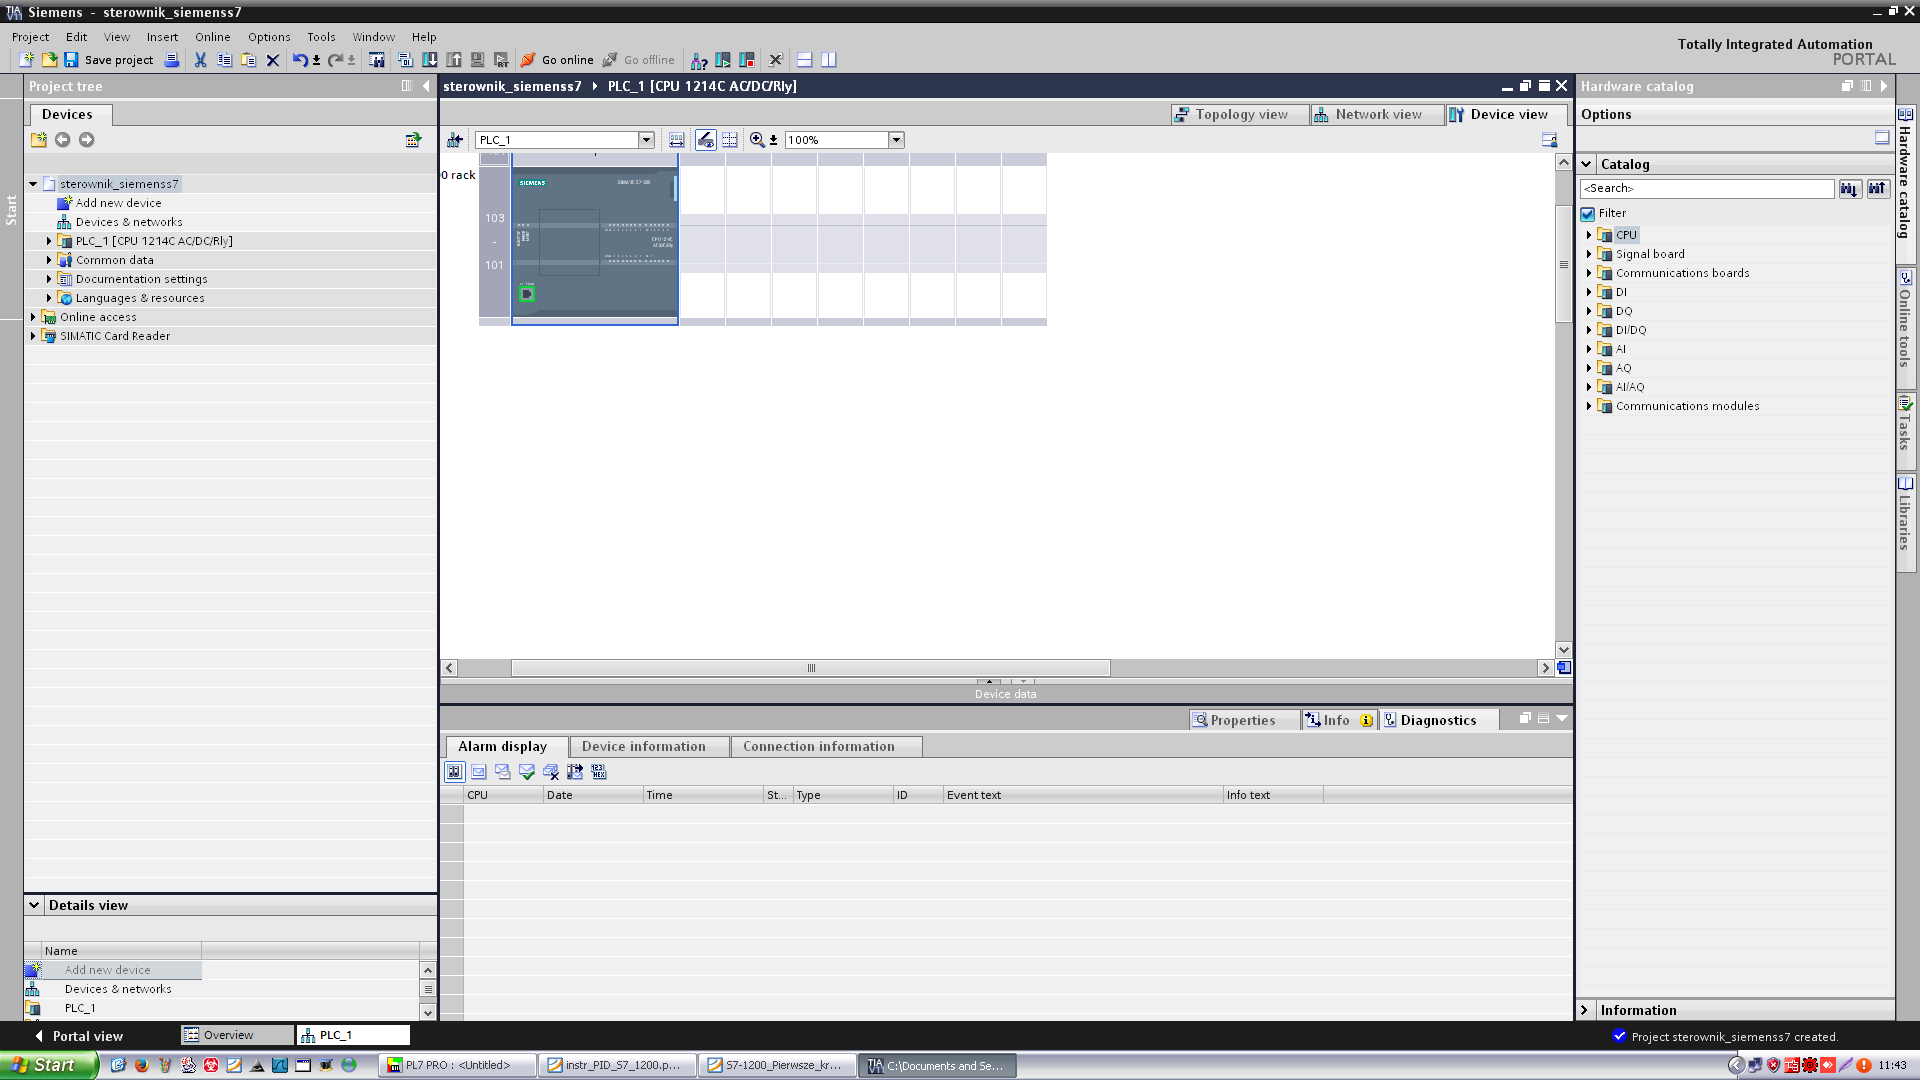
\includegraphics[scale=0.25]{./zdj/wstep.png}
        \caption{Automatycznie otwierane okno \textit{,,Device view''}}
        \label{device view}
    \end{figure}
    \begin{figure}[H]
        \centering
        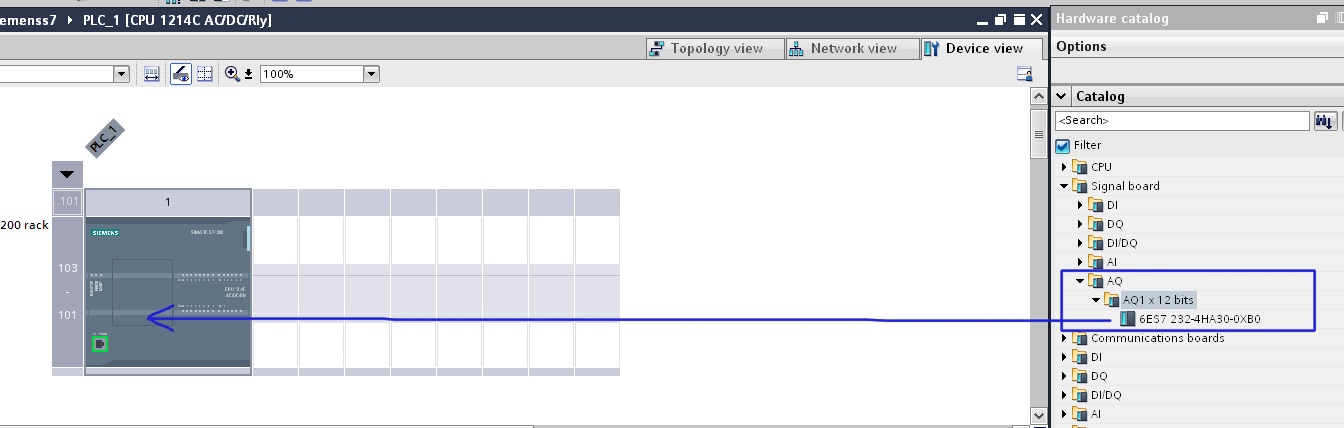
\includegraphics[scale=0.35]{./zdj/aq1_ok.png}
        \caption{Uzupełnienie konfiguracji sterownika o kartę sygnałową AQ1x12 }
        \label{aq1}
    \end{figure}

    \item Następnie, klikając w symbol złącza portu ethernetowego wywołuje się okno własności \textit{PROFINET interface\_1}, w którym nadano adres IP sterownika: 192.168.22.141 (rys. \ref{ip})
    \begin{figure}[H]
        \centering
        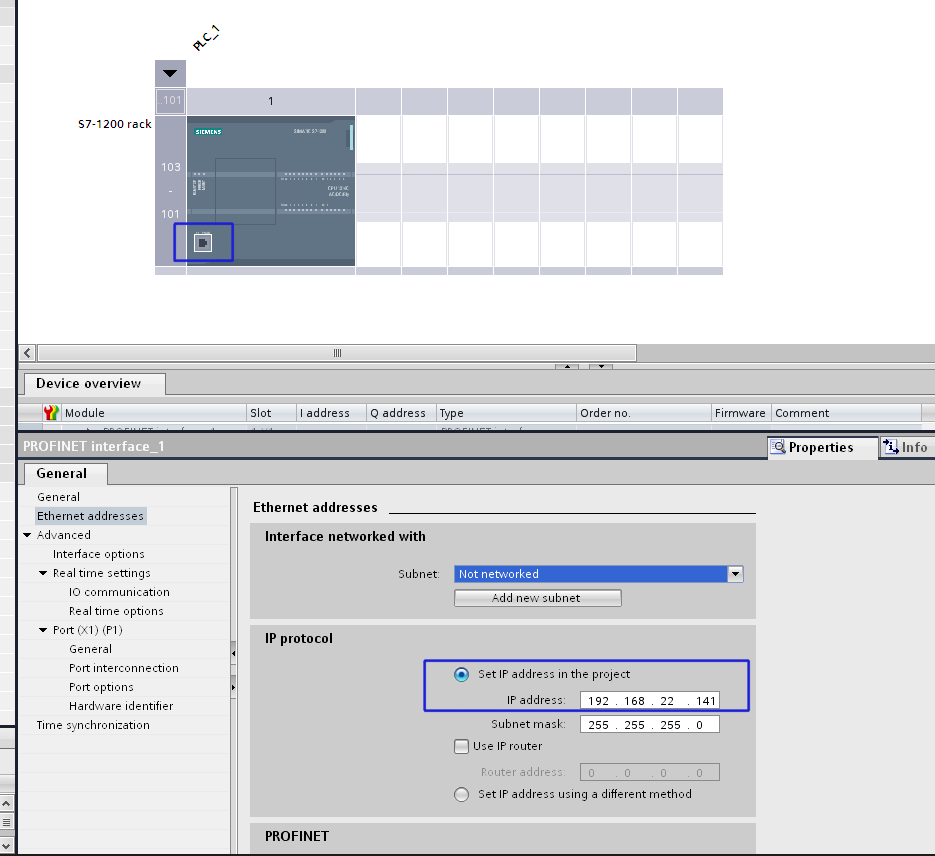
\includegraphics[scale=0.45]{./zdj/ip.png}
        \caption{Nadanie adresu IP sterownika}
        \label{ip}
    \end{figure}

    \item Ze względu na to, że później w programie będzie trzeba wykorzystać generator przebiegu zegarowego o częstotliwości 1Hz, uaktywniono go w zakładce ogólnych ustawień \textit{General $\rightarrow$ Pulse generators (PTO/PWM) $\rightarrow$ System and clock memory $\rightarrow$ Enable the use of clock memory byte} - rys. \ref{clock}.
    \begin{figure}[H]
        \centering
        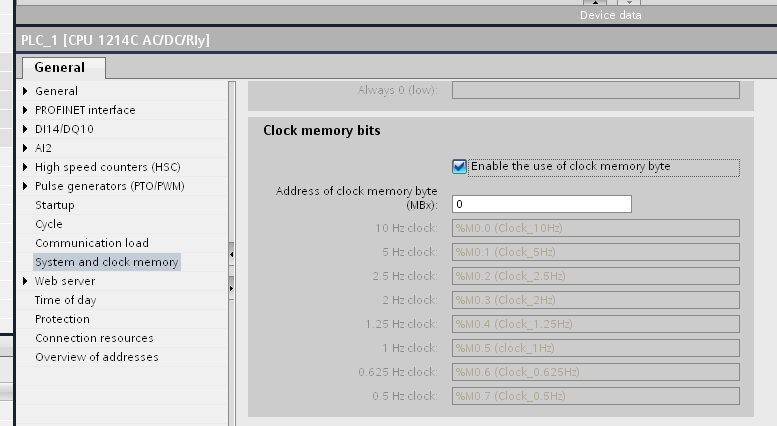
\includegraphics[scale=0.55]{./zdj/clock_bits.png}
        \caption{Uaktywnienie generatora przebiegu zegarowego}
        \label{clock}
    \end{figure} 

    \item Na koniec, aby sprawdzić, czy komputer poprawnie wyszukuje sterownik, posłużono się programem użytkowym S7-1200 Tool. Z listy wybrano odpowiedni adres IP, następnie w zakładce \textit{CPU} wybrano opcję \textit{Flash LED Lights}. Po wykonaniu tej czynności diody sterownika zaczęły mrugać, co oznaczało, że sterownik jest poprawnie wyszukiwany przez komputer. Na tym zakończyła się poprawna konfiguracja sterownika.
    \begin{figure}[H]
        \centering
        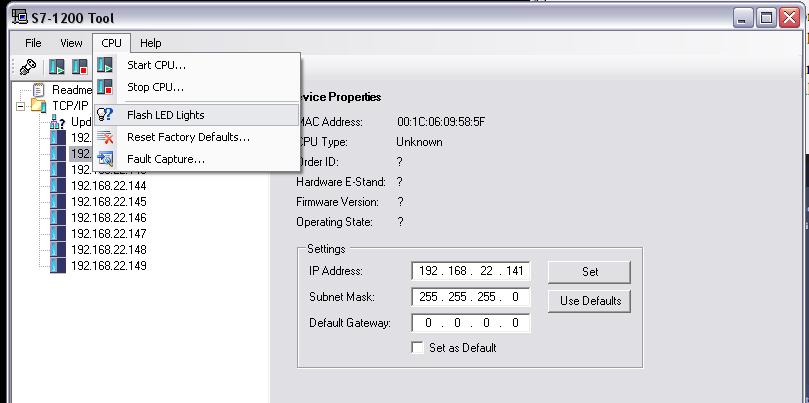
\includegraphics[scale=0.55]{./zdj/flash_led.png}
        \caption{Sprawdzenie podłączenia sterownika za pomocą programu S7-1200 Tool}
        \label{flash}
    \end{figure} 

\end{enumerate}

\section{Program w języku drabinkowym}
Tworzenie programu aplikacyjnego zaczyna się od wejścia w zakładkę \textit{Program
blocks} okna \textit{Project tree} i dwukrotnym kliknięciu w \textit{Main [OB1]}. Otworzy się okno do pisania programu w wybranym języku drabinkowym. Ponieważ program wynikowy ma się składać z dwóch podprogramów - mnożenia dwóch liczb oraz licznika, należy stworzyć dwa osobne bloki. W tym celu należało w zakładce \textit{Program blocks} wybrać opcję \textit{Add new block}. Po wyświetleniu okna jak na rys. \ref{bloki}, należało wybrać opcję \textit{Function} oraz wpisać nazwę funkcji. W ten sposób utworzono dwa osobne podprogramy - mnożenie oraz licznik.

\begin{figure}[H]
    \centering
    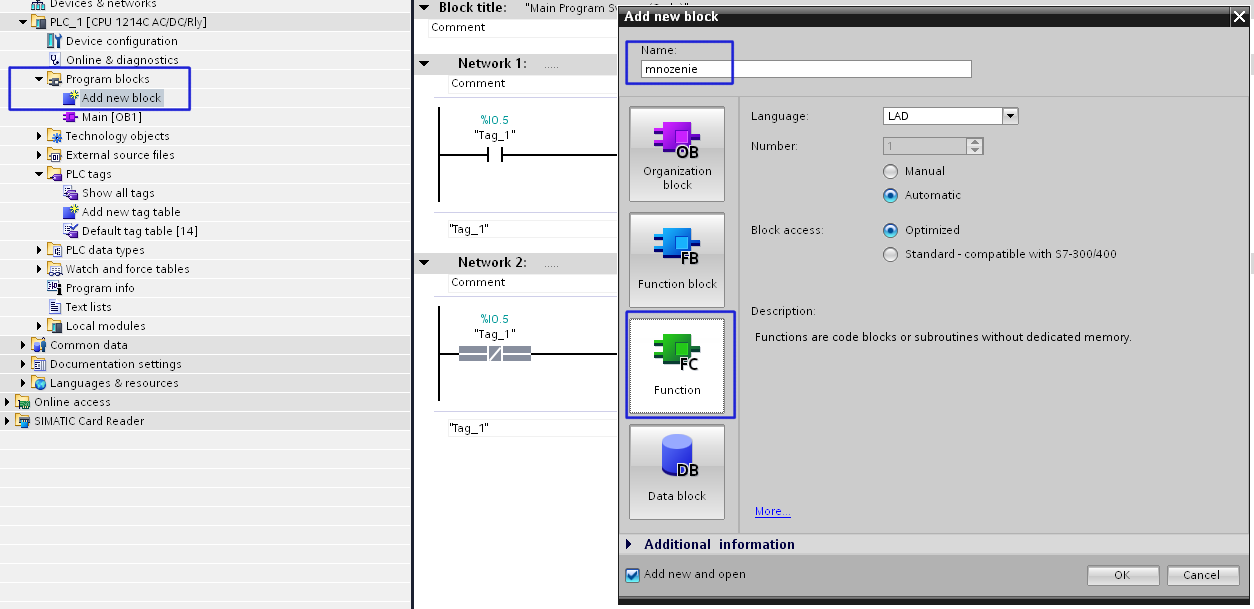
\includegraphics[scale=0.4]{./zdj/blok_mnozenie.png}
    \caption{Tworzenie funkcji}
    \label{bloki}
\end{figure} 


\subsection{Program główny}
Program główny składa się z dwóch podprogramów - mnożenia oraz licznika. Na zdjęciu \ref{main} przedstawiono jak wygląda program główny. Składa się z dwóch gałęzi (networks). Wejście analogowe $\%I0.5$ decyduje o tym, który podprogram ma się uruchomić.
\begin{figure}[H]
    \centering
    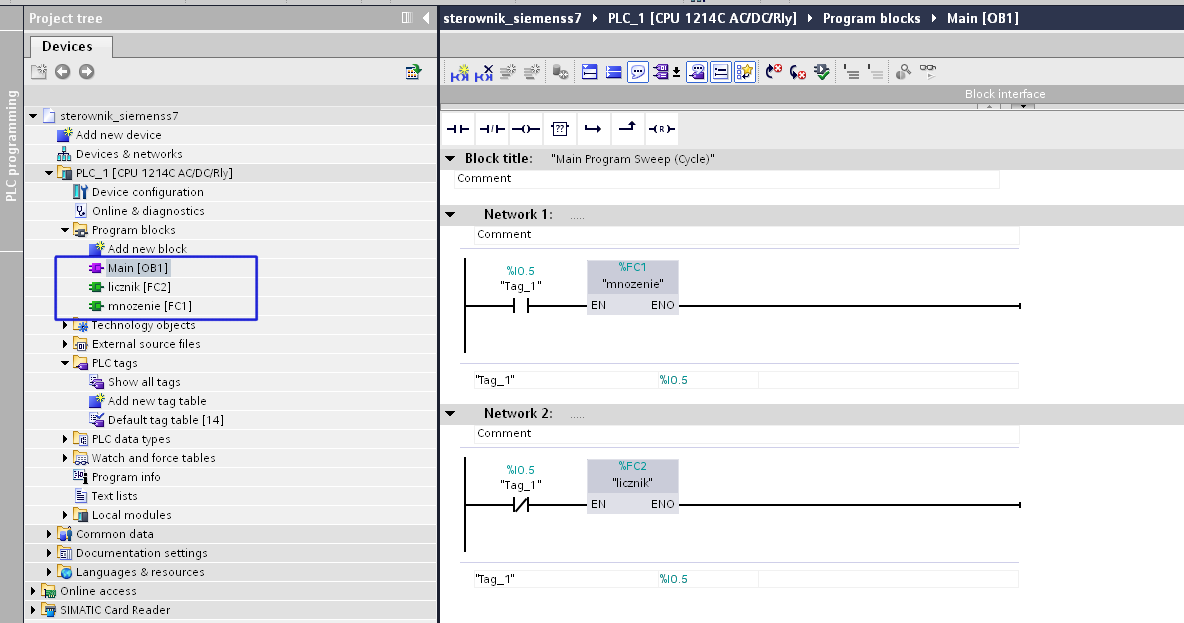
\includegraphics[scale=0.4]{./zdj/main.png}
    \caption{Program główny}
    \label{main}
\end{figure} 

\subsection{Mnożenie dwóch liczb}
Program mnożenia dwóch liczb składa się z 3 gałęzi (networks). Pierwsza gałąź, przedstawiona na rys. \ref{network1}, zajmuje się odczytaniem pierwszej liczby, która ma być podstawiona za ,,x''. Ta część programu uruchamia się tylko, gdy obsługiwane jest wejście analogowe $\%I0.0$. W zależności od tego, ile razy zwarte zostanie to wejście, taką wartość przyjmie ,,x''. Ta część programu wykorzystuje licznik, który zlicza liczbę zwarcia wejścia oraz blok ,,move'', który tę liczbę wyświetla na wyjście $\%QB0$. Analogicznie działa gałąź druga (rys. \ref{network2}), która zlicza liczbę zwarć wejścia $\%I0.1$ i tę wartość przypisuje do ,,y'' i pokazuje na wyjściu $\%QB0$. 

\begin{figure}[H]
    \centering
    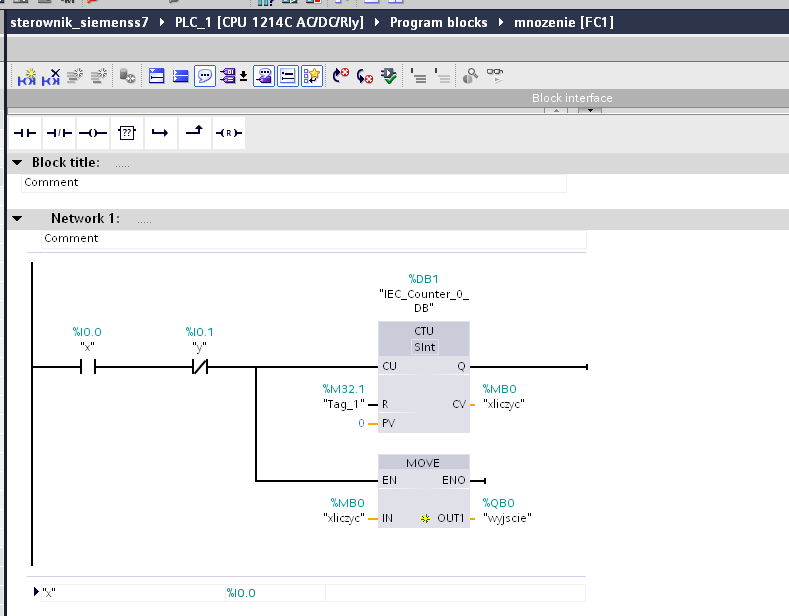
\includegraphics[width=\textwidth]{./zdj/network1.png}
    \caption{Gałąź pierwsza programu mnożenia dwóch liczb}
    \label{network1}
\end{figure} 

\begin{figure}[H]
    \centering
    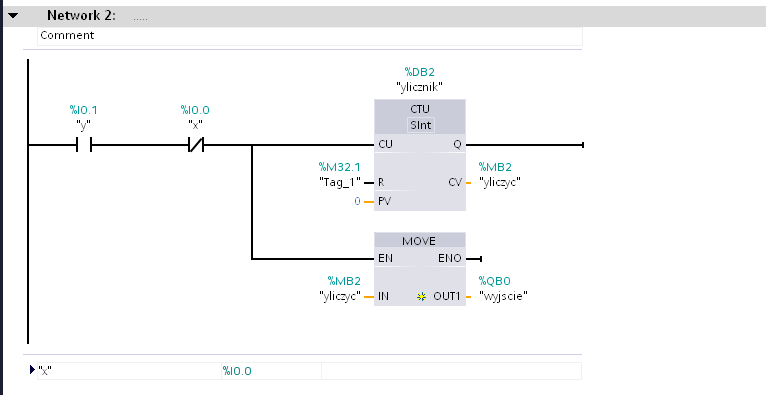
\includegraphics[width=\textwidth]{./zdj/network2.png}
    \caption{Gałąź druga programu mnożenia dwóch liczb}
    \label{network2}
\end{figure} 

Trzecia gałąź programu wykorzystuje blok ,,mul'', służący do wymnażania podanych na wejście liczb (,,x'', ,,y''). Wynik mnożenia zapisuje do zmiennej ,,z'' i wyświetla na wyjściu $\%QB0$. 

\begin{figure}[H]
    \centering
    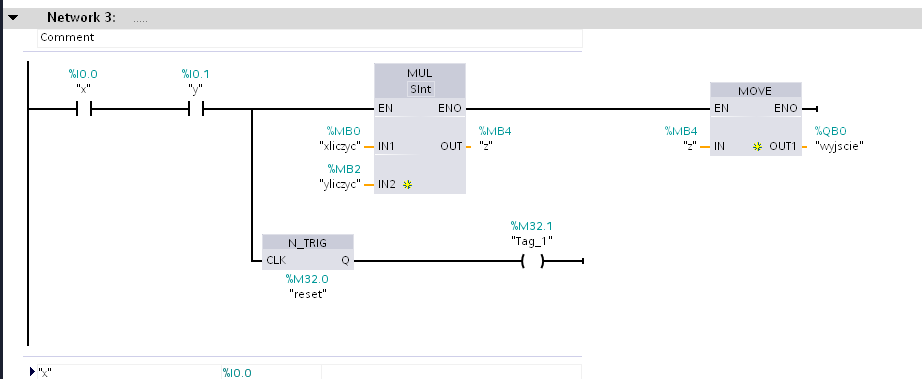
\includegraphics[width=\textwidth]{./zdj/network3.png}
    \caption{Gałąź trzecia programu mnożenia dwóch liczb}
    \label{network3}
\end{figure} 



\subsection{Licznik}
Na zdjęciu \ref{licznik} przedstawiono program licznika. Wykorzystuje on generator przebiegu zegarowego o częstotliwości 1 Hz oraz blok licznika, który zlicza w górę lub w dół w zakresie od 0 do 10.

\begin{figure}[H]
    \centering
    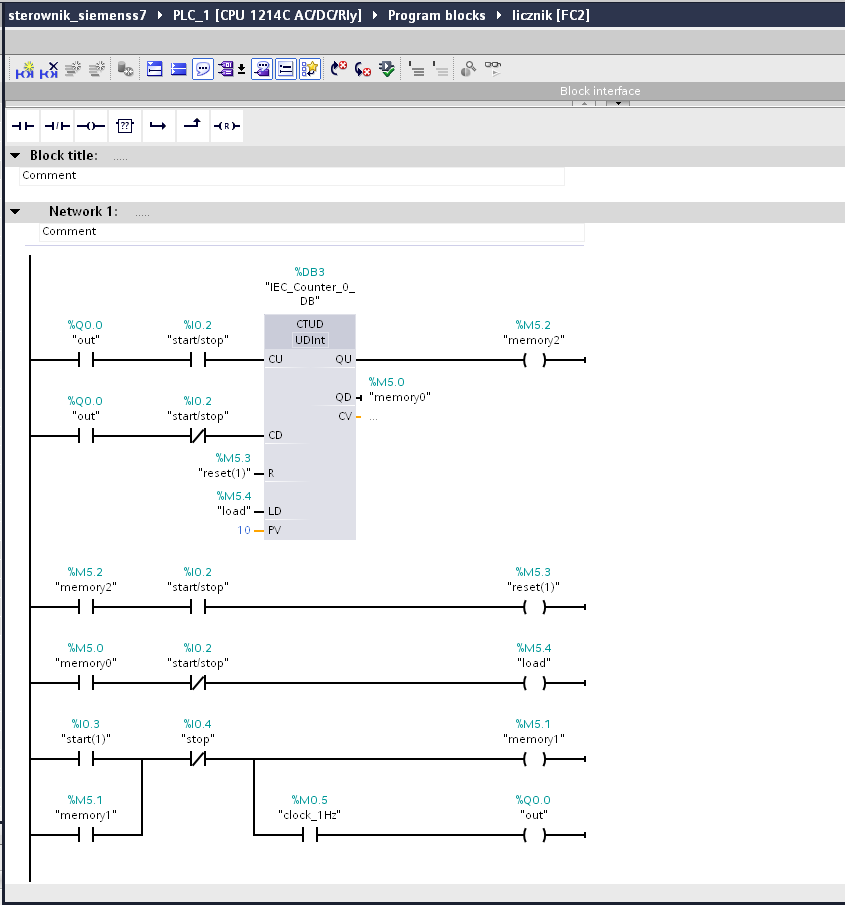
\includegraphics[width=\textwidth]{./zdj/licznik.png}
    \caption{Program licznika}
    \label{licznik}
\end{figure} 


\subsection{Kompilacja i przesłanie programu do sterownika}
W celu przesłania programu do sterownika należy najpierw kliknąć prawym przyciskiem na ,,PLC\_1'' w zakładce \textit{Project tree}, po czym wybrać opcję kompilacji \textit{Compile $\rightarrow$ All}. Na zdjęciu \ref{kompilacja} przedstawiono poprawnie skompilowany program.

\begin{figure}[H]
    \centering
    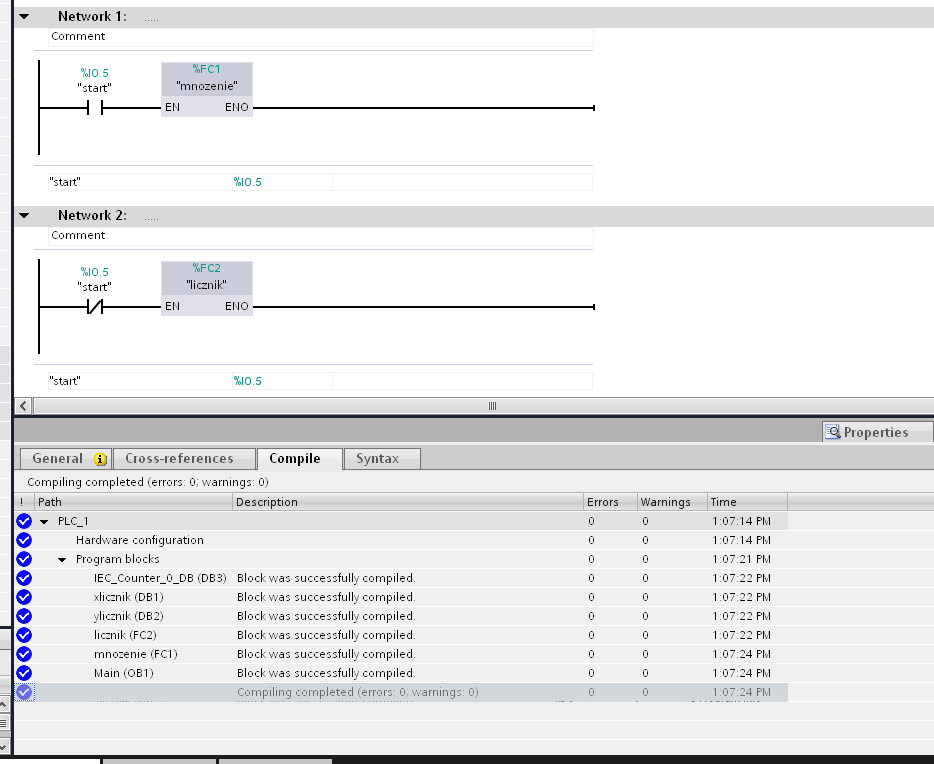
\includegraphics[width=\textwidth]{./zdj/kompilacja.png}
    \caption{Poprawnie skompilowany program}
    \label{kompilacja}
\end{figure} 

Po udanej kompilacji można przesłać program do sterownika. W tym celu należy kliknąć \textit{Download to device $\rightarrow$ All}. Proces przesyłania przedstawiono na rys. \ref{przesylanie}.

\begin{figure}[H]
    \centering
    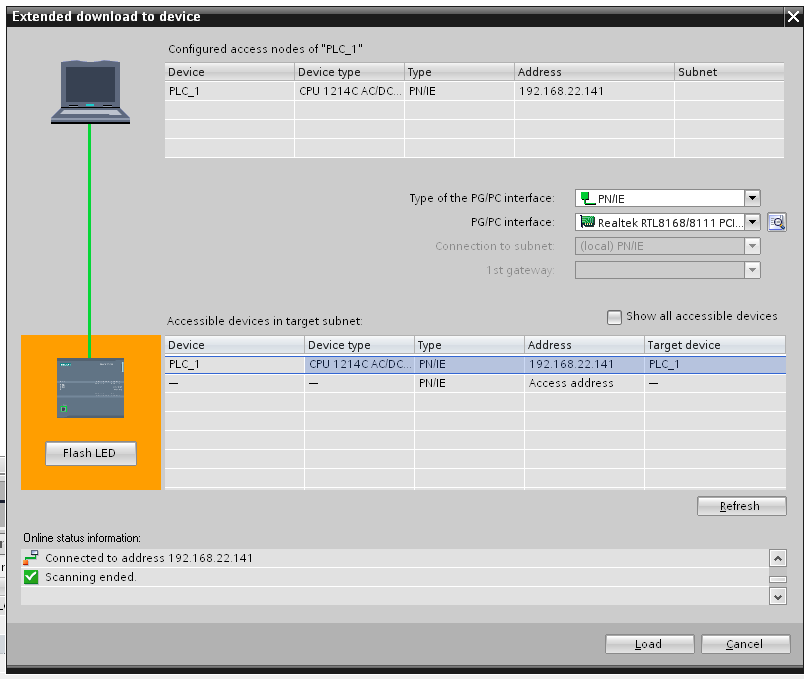
\includegraphics[width=\textwidth]{./zdj/przesylanie.png}
    \caption{Przesyłanie programu do sterownika}
    \label{przesylanie}
\end{figure} 

Po poprawnym przesłaniu programu do sterownika, należy kliknąć opcję \textit{Go online} i \textit{Monitoring} (ikona okularów), które umożliwią śledzenie wykonywania programu w czasie rzeczywistym w programie.

\subsection{Testowanie działania programu}
\subsubsection{Mnożenie dwóch liczb}

W celu przetestowania programu mnożenia dwóch liczb zwarto wejście $\%I0.5$. Następnie zwierano wejście $\%I0.0$ np. 5 razy (fizycznie wyciągano i wkładano przewód do wejścia $\%I0.0$) i rozwarto. W gałęzi pierwszej programu można było zauważyć, że pod ,,x'' wpisana została wartość 5 (rys. \ref{mnozenie_test1}), została ona także wyświetlona na sterowniku na wyjściu $\%QB0$. Potem zwierano wejście $\%I0.1$ np. 8 razy. Za ,,y'' podstawiona została wartość 8 (rys. \ref{mnozenie_test2}) i wyświetliła się na sterowniku na wyjściu $\%QB0$. Następnie zwarto obydwa wejścia $\%I0.0$ oraz $\%I0.1$ i uzyskano wynik mnożenia - liczbę 40 wyświetloną w programie (rys. \ref{mnozenie_test3}) oraz na sterowniku na wyjściu $\%QB0$.

\begin{figure}[H]
    \centering
    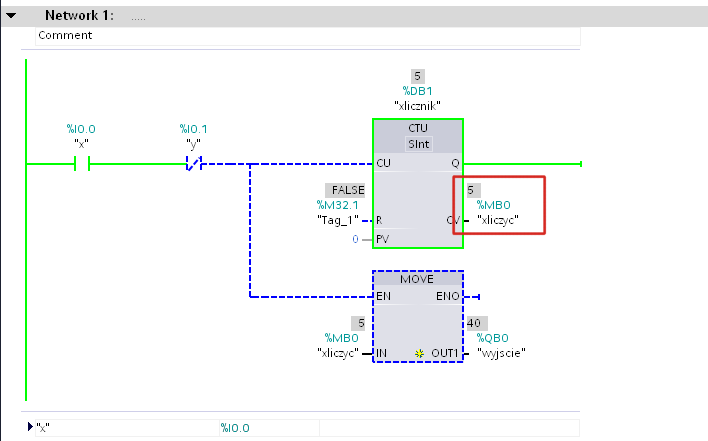
\includegraphics[width=\textwidth]{./zdj/mnozenie_test1.png}
    \caption{Wartość x}
    \label{mnozenie_test1}
\end{figure} 

\begin{figure}[H]
    \centering
    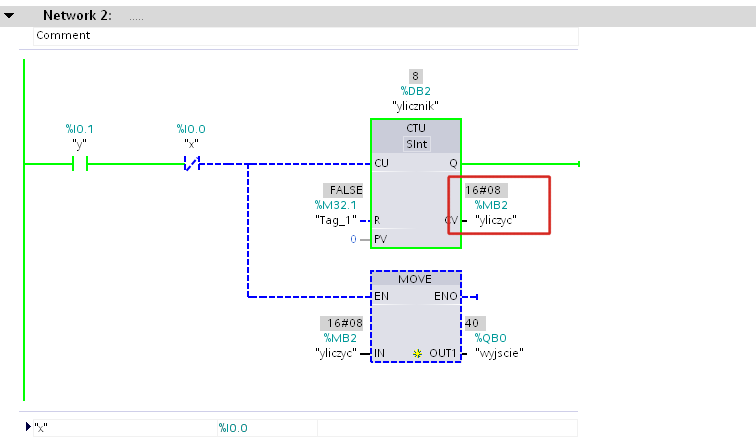
\includegraphics[width=\textwidth]{./zdj/mnozenie_test2.png}
    \caption{Wartość y}
    \label{mnozenie_test2}
\end{figure} 

\begin{figure}[H]
    \centering
    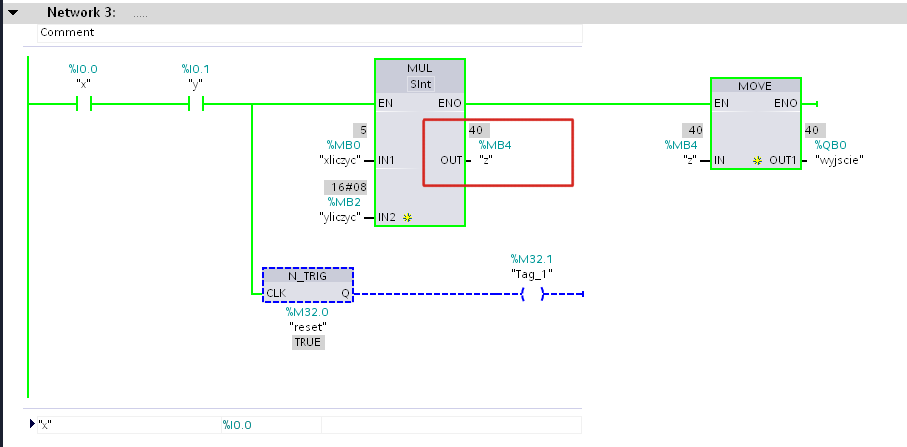
\includegraphics[width=\textwidth]{./zdj/mnozenie_test3.png}
    \caption{Wynik mnożenia}
    \label{mnozenie_test3}
\end{figure} 




\subsubsection{Licznik}
W celu przetestowania programu licznika rozwarto wejście $\%I0.5$. Następnie w celu uruchomienia licznika, należało zewrzeć wejście $\%I0.3$, które generuje przebieg oraz uruchamia licznik. Zwarcie wejścia $\%I0.4$ zatrzymuje licznik. Zwarcie wejścia $\%I0.2$ rozpoczynało zliczanie w górę przez licznik w zakresie od 0 do 10. Natomiast rozwarcie wejścia $\%I0.4$ rozpoczynało zliczanie w dół przez licznik w zakresie od 10 do 0.
\begin{figure}[H]
    \centering
    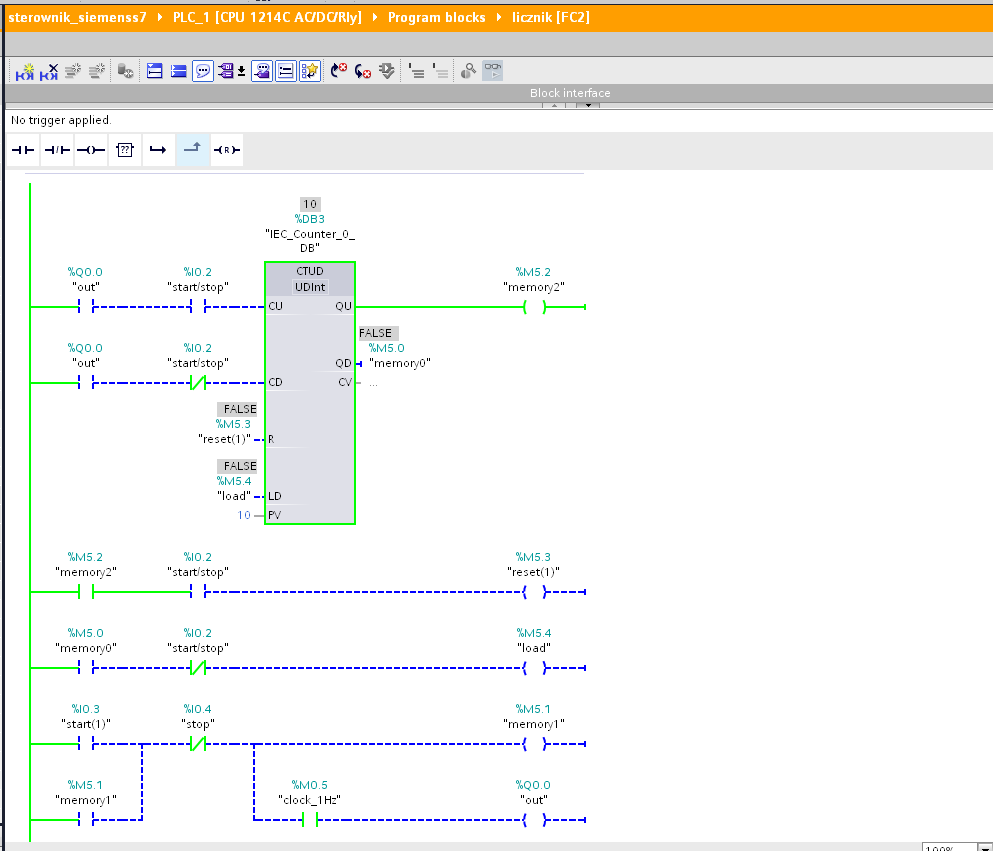
\includegraphics[width=\textwidth]{./zdj/licznik_test.png}
    \caption{Testowanie programu licznika}
    \label{licznik_test}
\end{figure} 




\section{Podsumowanie}
Ćwiczenie pozwoliło zapoznać się z obsługą sterownika Siemens Simatic S7-1200 poprzez program TIA Portal 11. Konfiguracja sterownika oraz napisanie i uruchomienie programów nie przysporzyło większych problemów. Obydwa programy działały zgodnie z założeniami.



\end{document}